\documentclass[titlepage, letterpaper, 10.5pt]{article}
\usepackage[letterpaper, margin=1.25in]{geometry}
\usepackage{graphicx}
\usepackage{comment}
\usepackage{amsmath}
\usepackage{caption}
\usepackage{subcaption}
\usepackage{nicefrac}
\usepackage{verbatim}
\usepackage{tablefootnote}

\begin{document}

\title{Phase Locked Loop}
\author{Ben Lorenzetti}
\date{Start Date: April 2, 2015\\
Submission Date: April 20, 2015}
\maketitle

\clearpage
\mbox{}
\thispagestyle{empty}
\clearpage
\setcounter{page}{1}

\tableofcontents

\section{Objective}

To measure the characteristics of a phase locked loop and to investigate and model its behavior in an FSK (frequency-shift keying) demodulator.

\clearpage
\section{Principles of Operation}
\label{principles-of-operation}

\begin{figure}[ht]
	\centering
	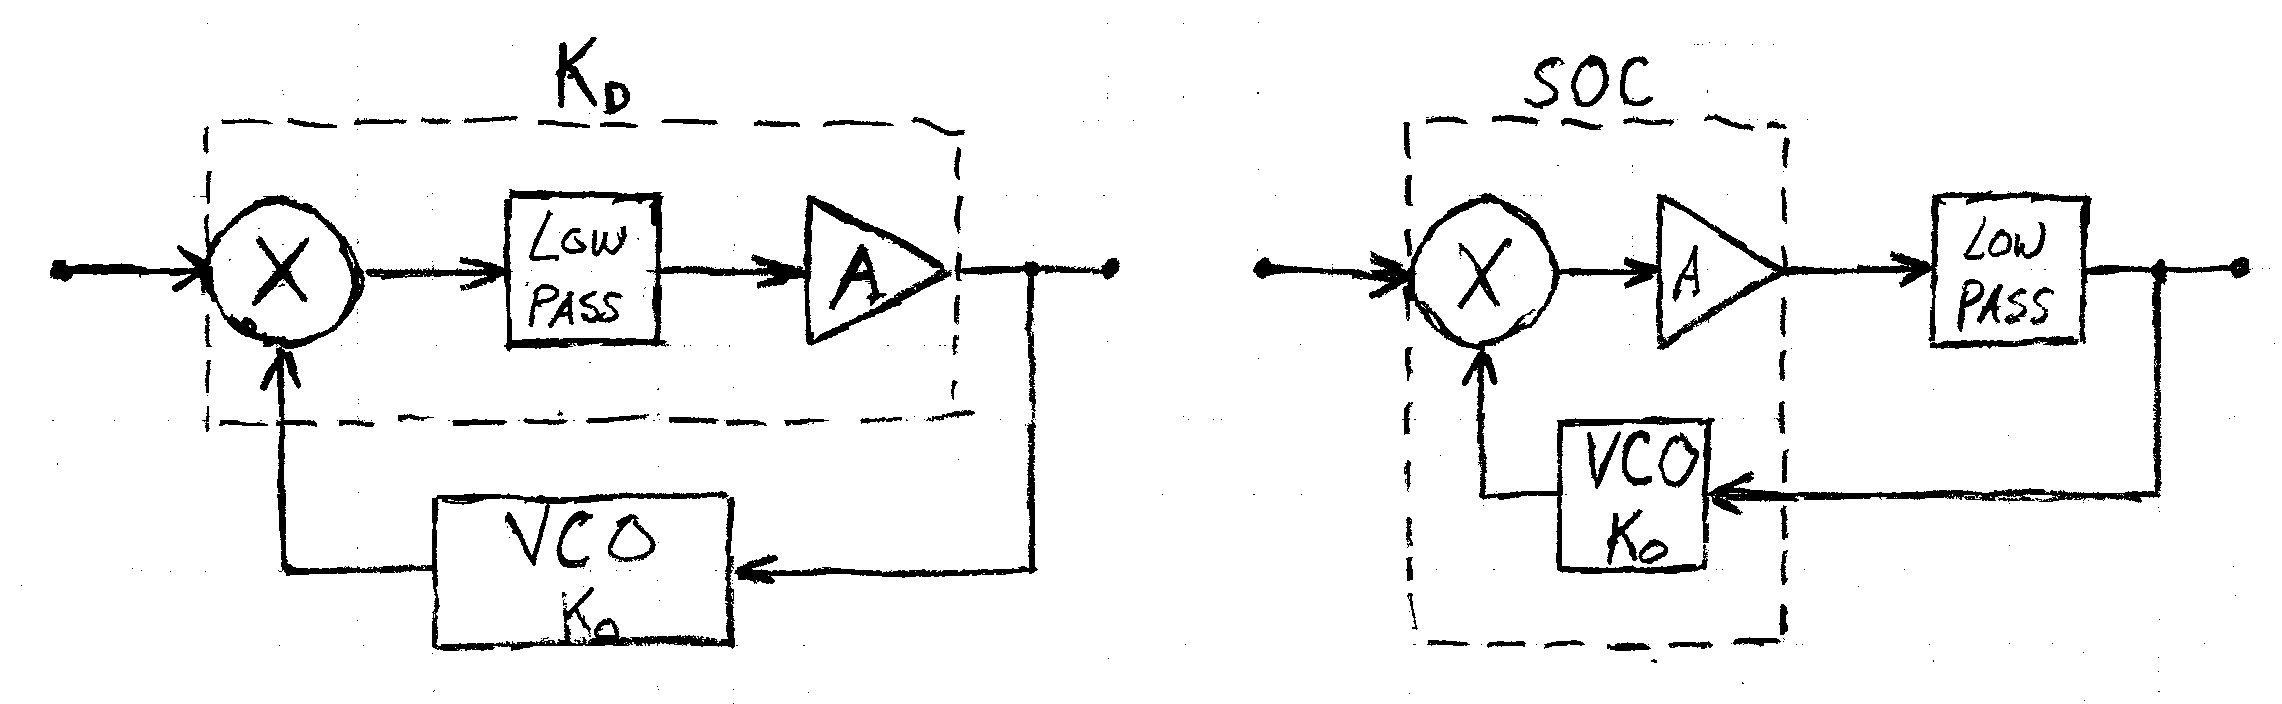
\includegraphics[width=0.7\textwidth]{diagrams/pll-demodulator-block-diagram}
	\caption{PLL Demodulator Block Diagram (left); Rearrangement for SOC Integration (right).}
	\label{pll-demodulator-block-diagram}
\end{figure}

\clearpage
\section{Theory}

\subsection{Texas Instruments LM656}

\begin{figure}[ht]
	\centering
	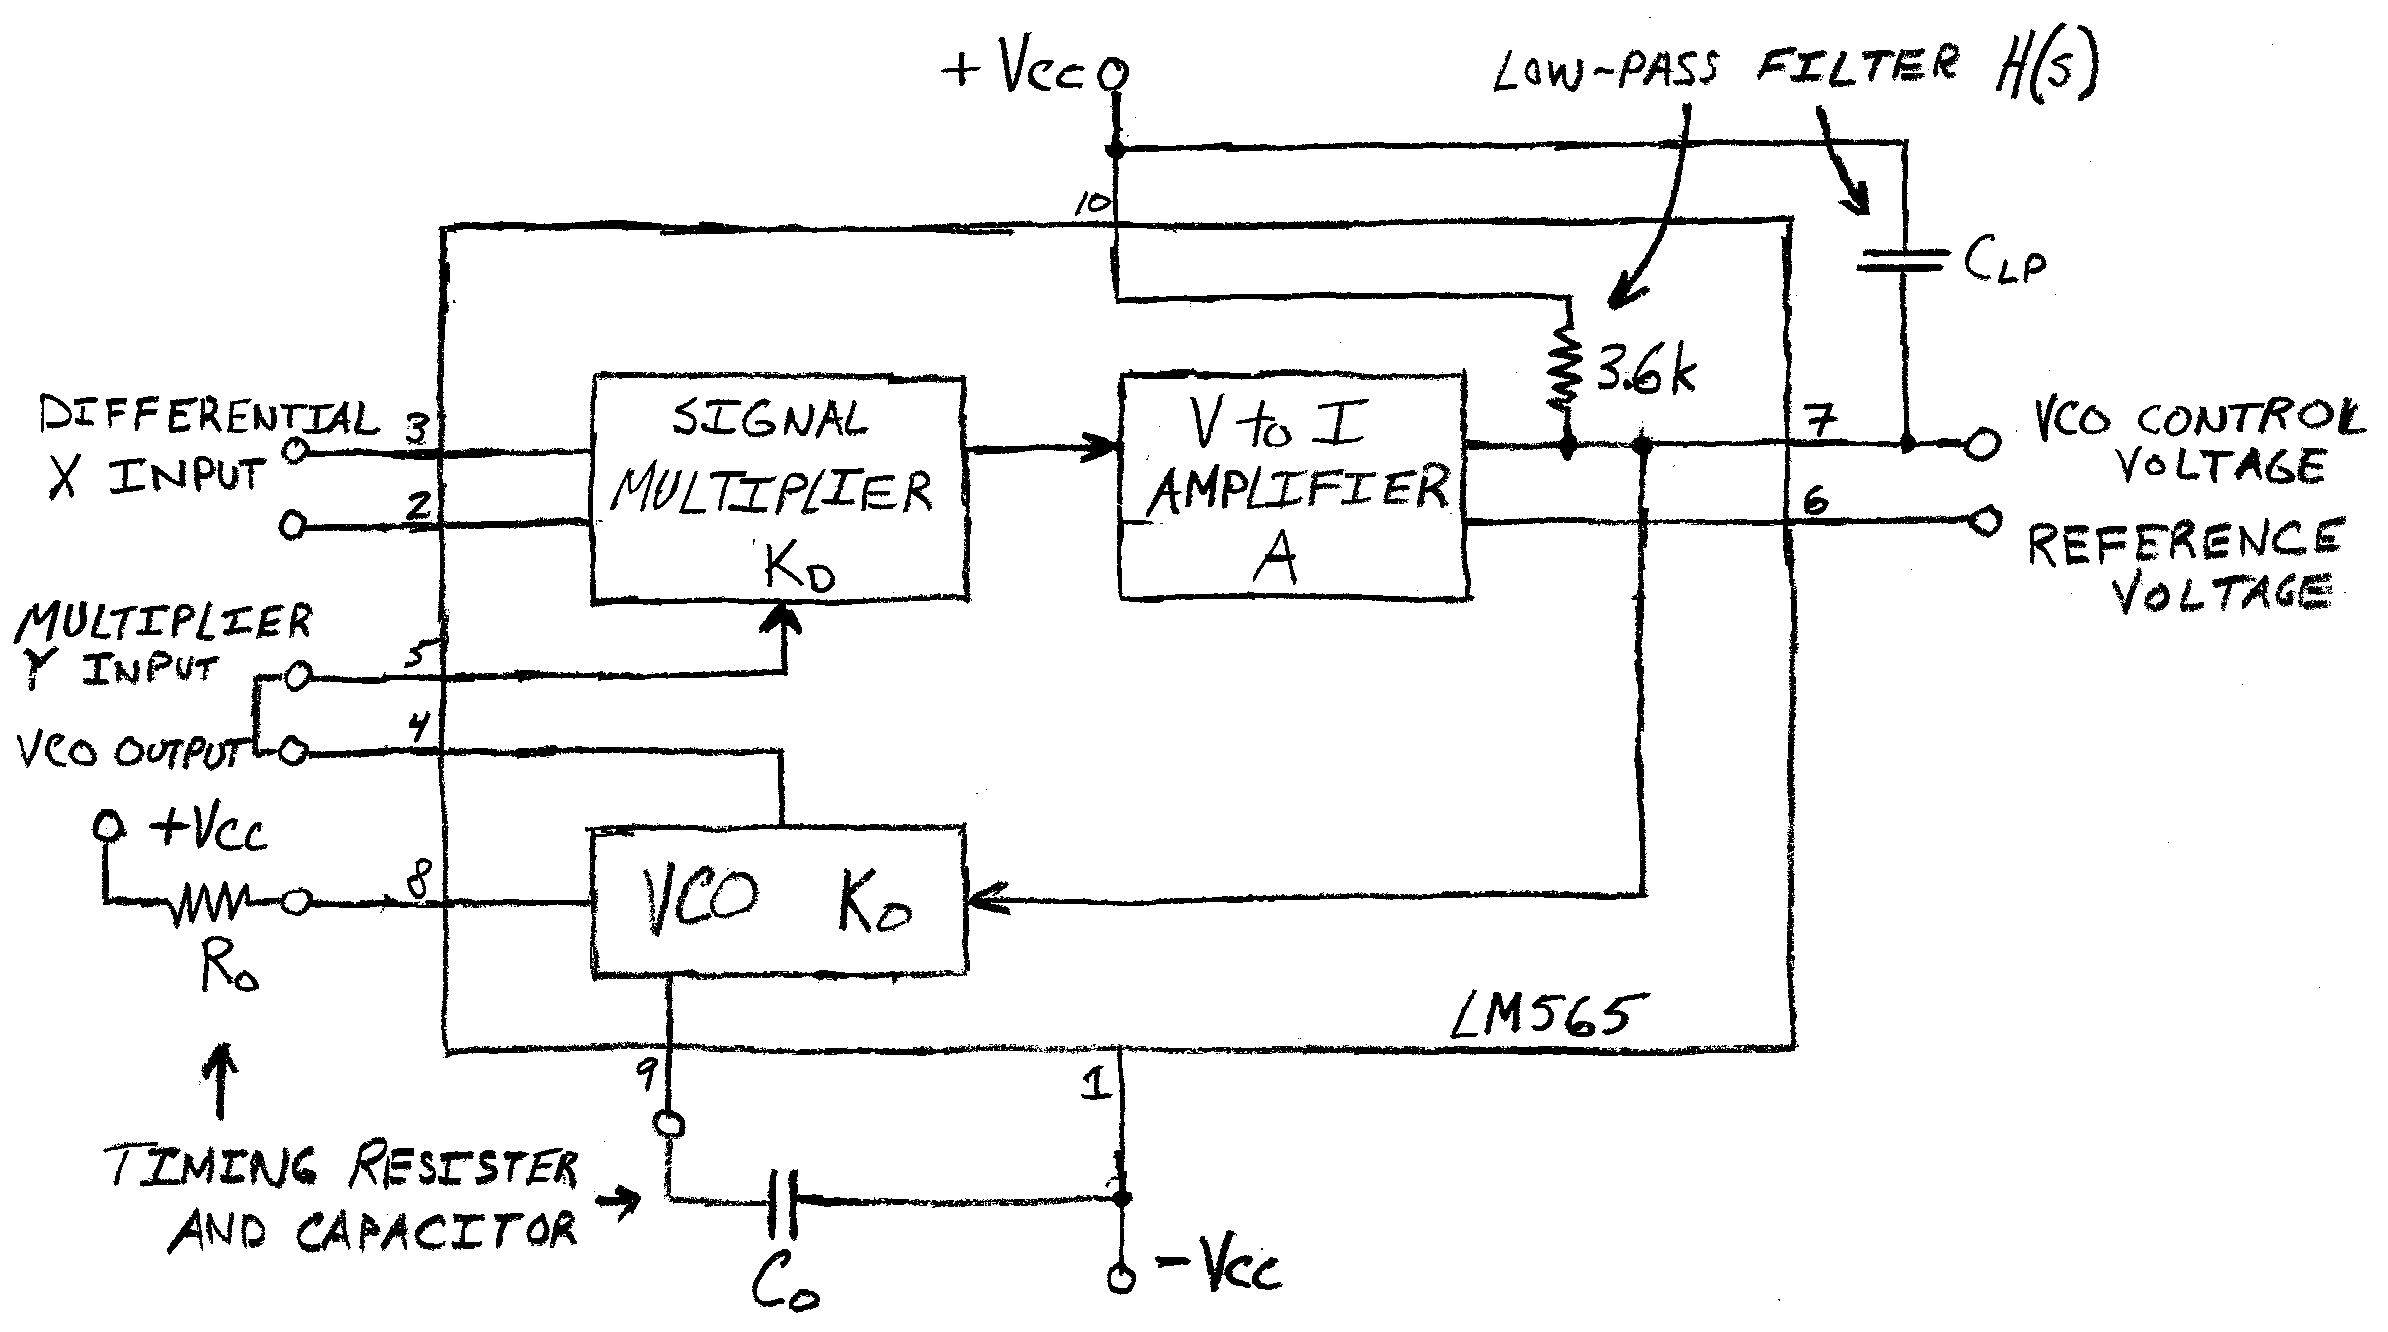
\includegraphics[width=0.75\textwidth]{diagrams/565-block-diagram}
	\caption{Rough Block Diagram for the LM565 Phase Locked Loop}
	\label{565-block-diagram}
\end{figure}

As discussed in the section \ref{principles-of-operation}, most of a PLL demodulator can be integrated onto a single silicon wafer--called a system-on-a-chip (SOC).
The only parts that cannot be fabricated on silicon are the capacitors, so the PLL demodulator has been redesigned with this in mind.
A company called Signetics was the first to put a PLL on an SOC, but they are out of business so we have a similar chip from Texas Instruments, the LM565.

The LM565 makes it easy for the circuit designer to incorporate frequency-shift keying into their product; you just have to slap on a few capacitors to have a working demodulator.
The only design that must be done is selecting a free-running frequency $f_{0}$ near the transmission frequency and building a low-pass filter with bandwidth greater than the frequency shift but less than twice the transmission frequency.
Use the following equation from the LM565 datasheet to select $f_{0}$.
\begin{equation}
f_{0}=\frac{0.3}{R_{0}C_{0}}
\label{f0-eq}
\end{equation}

For more information about how the LM565 works, see the schematic diagram in section \ref{lm565-schematic-diagram}.

\clearpage
\subsection{Voltage Controlled Oscillator}

\begin{figure}[ht]
	\centering
	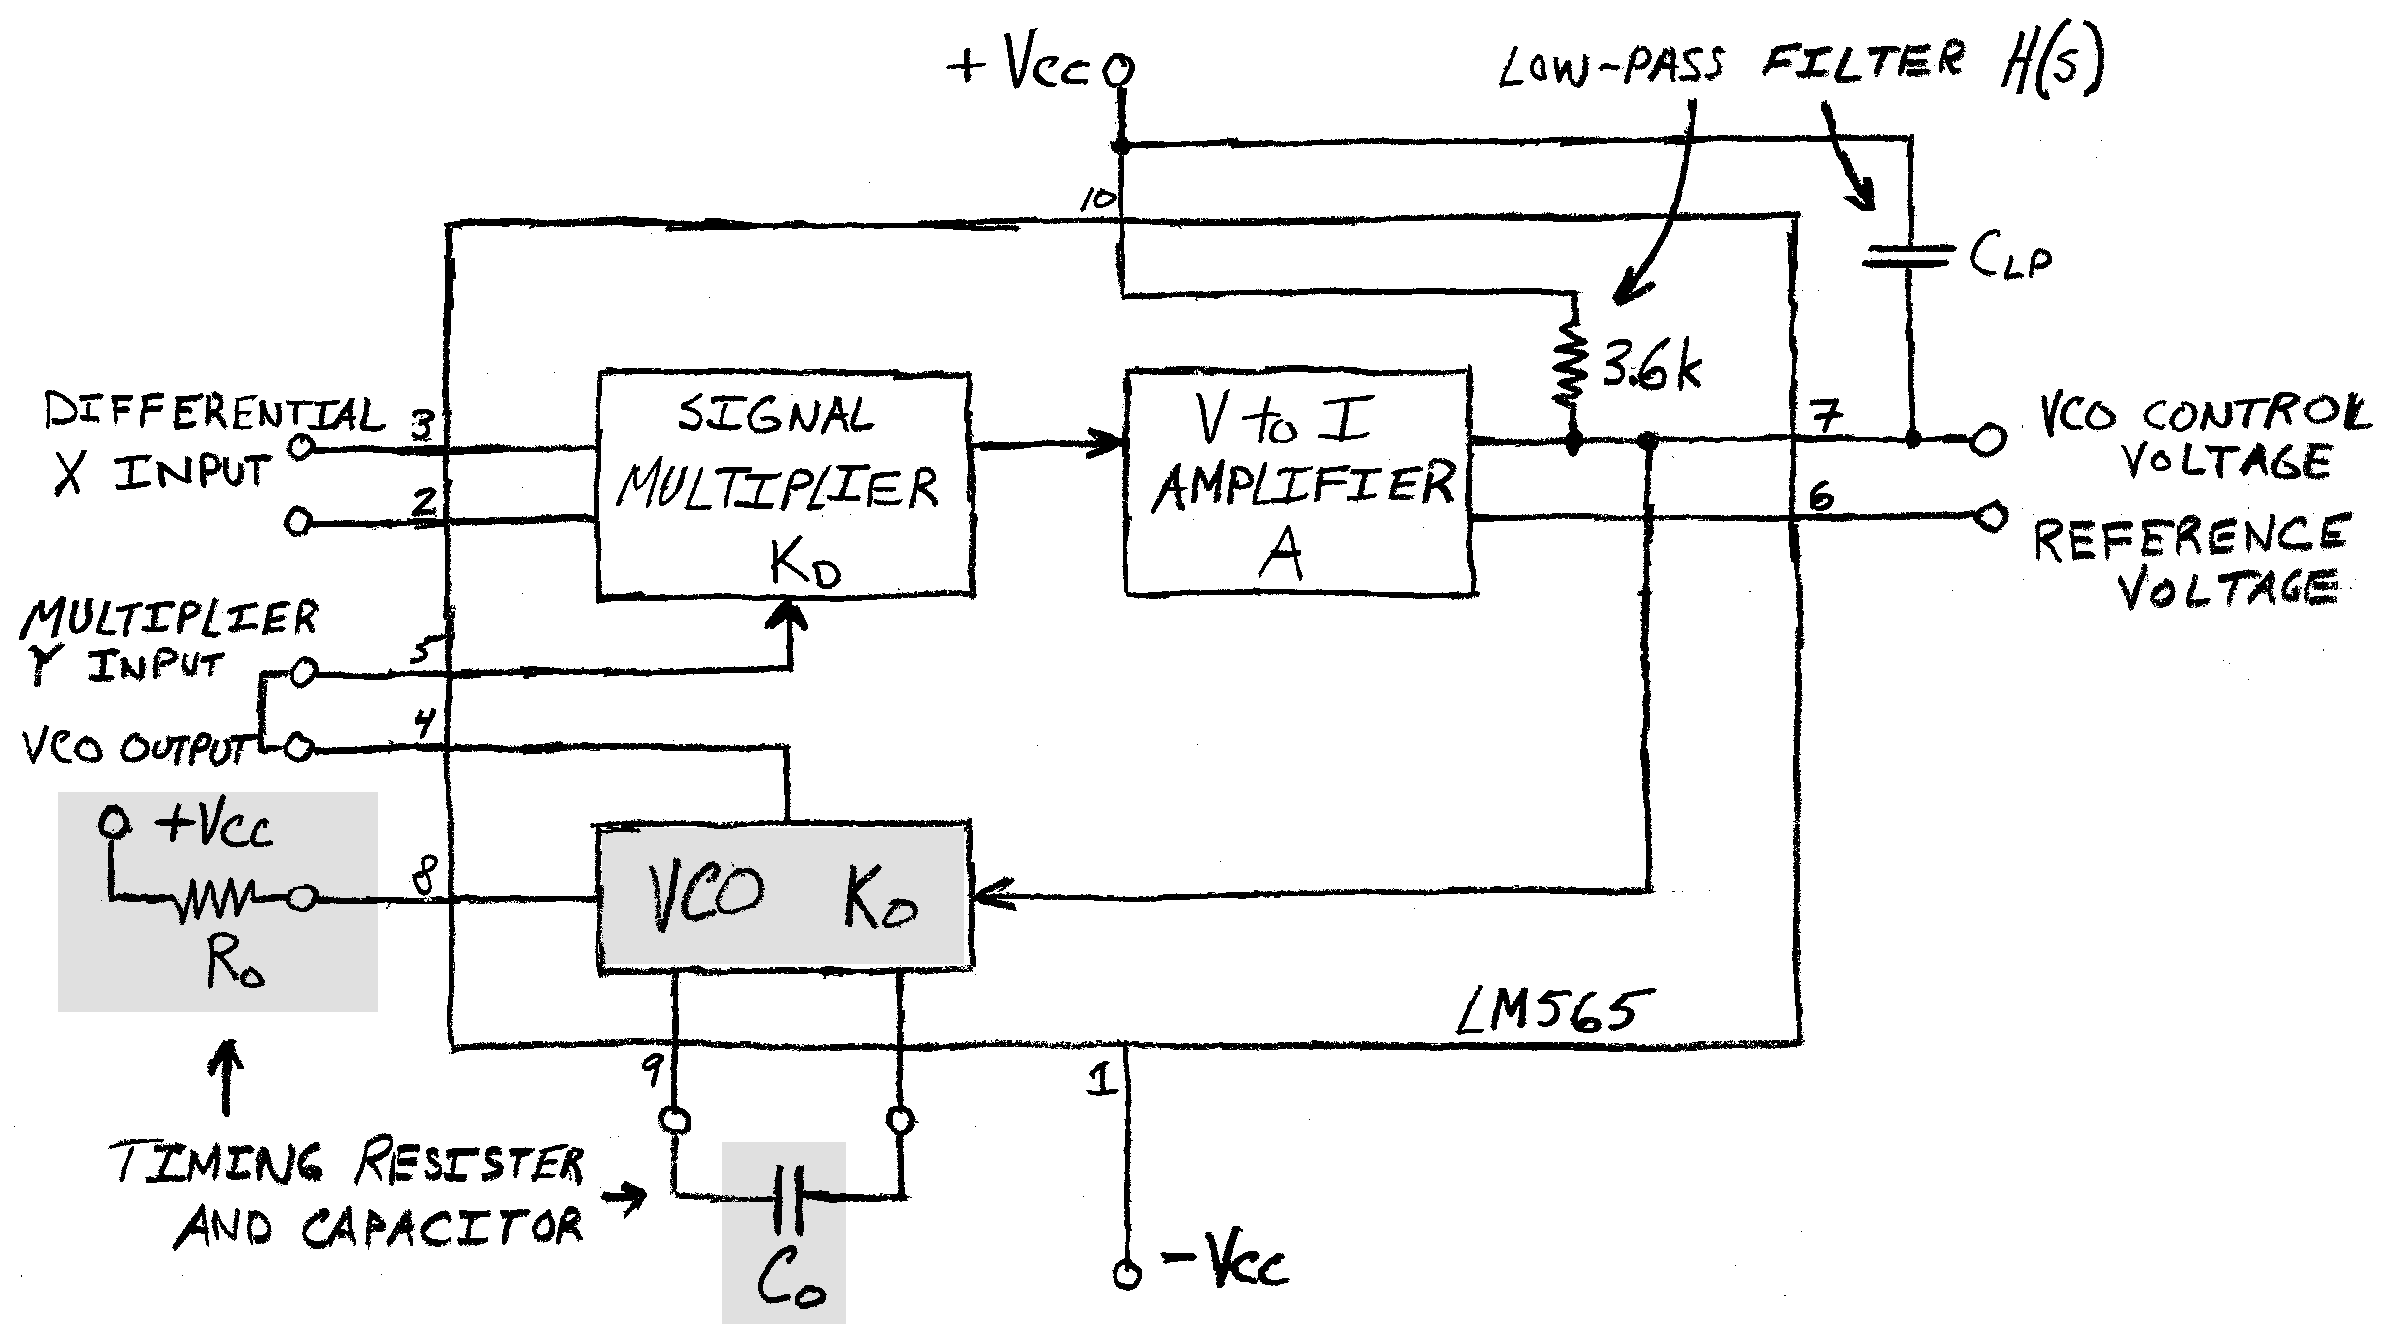
\includegraphics[width=0.75\textwidth]{diagrams/565-block-diagram-vco}
	\caption{Role of the Voltage Controlled Oscillator in the LM565 PLL}
	\label{565-block-diagram-vco}
\end{figure}

\clearpage
\subsection{Signal Multiplier}

\begin{figure}[ht]
	\centering
	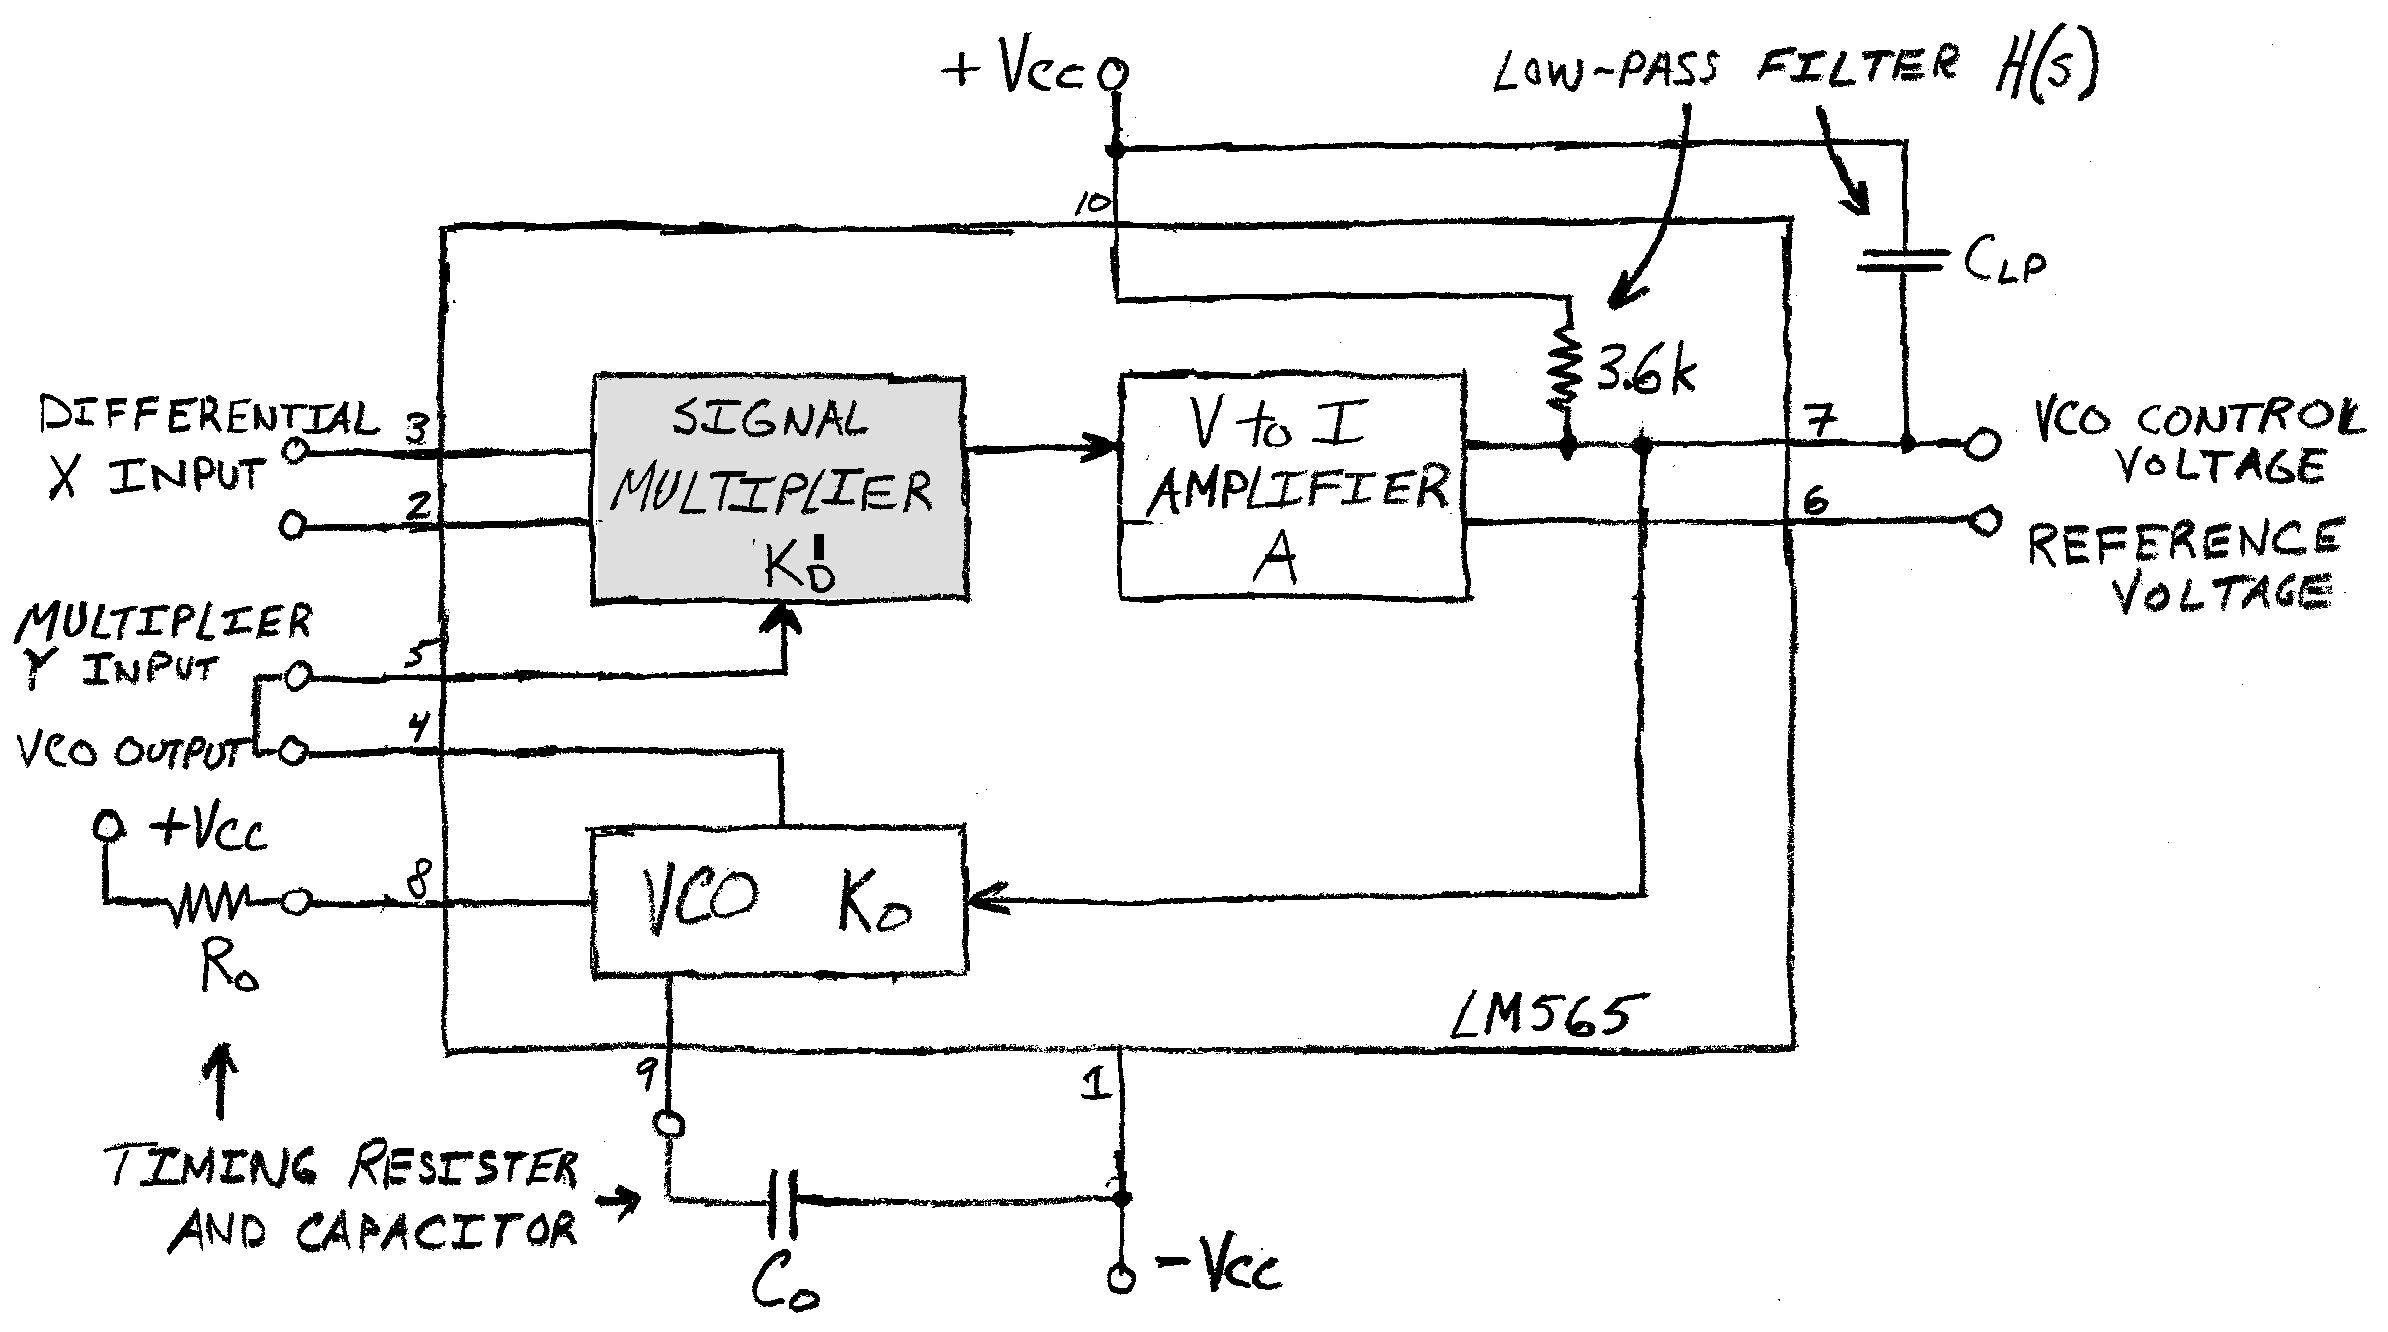
\includegraphics[width=0.75\textwidth]{diagrams/565-block-diagram-signal-multiplier}
	\caption{Role of the Multiplier/Mixer/Phase Detector in the LM565 PLL}
	\label{565-block-diagram-signal-multiplier}
\end{figure}


Addition and subtraction are easy in electronics; just use a shunt or series connection, depending on whether you are summing current or voltage.
Multiplication is more difficult; there is no obvious way to mix two signals.

A first though for inplementing a multiplier is to look at the problem in frequency domain and see if that offers any insight.
The fourier transform of multiplication is
\begin{equation*}
x(t)y(t) \Longleftrightarrow X(s)*Y(s)
\end{equation*}

This is not very helpful because thinking about designing a frequency convolution device is even worse than a signal multiplier.
However, there is another mathmatics formula that can give us an implementation idea: the addition propery of logarithms.
\begin{equation}
ln(x)+ln(y)=ln(x\times y)
\label{log-eq}
\end{equation}

\clearpage
\subsection{Transconductance Amplifier}

\begin{figure}[ht]
	\centering
	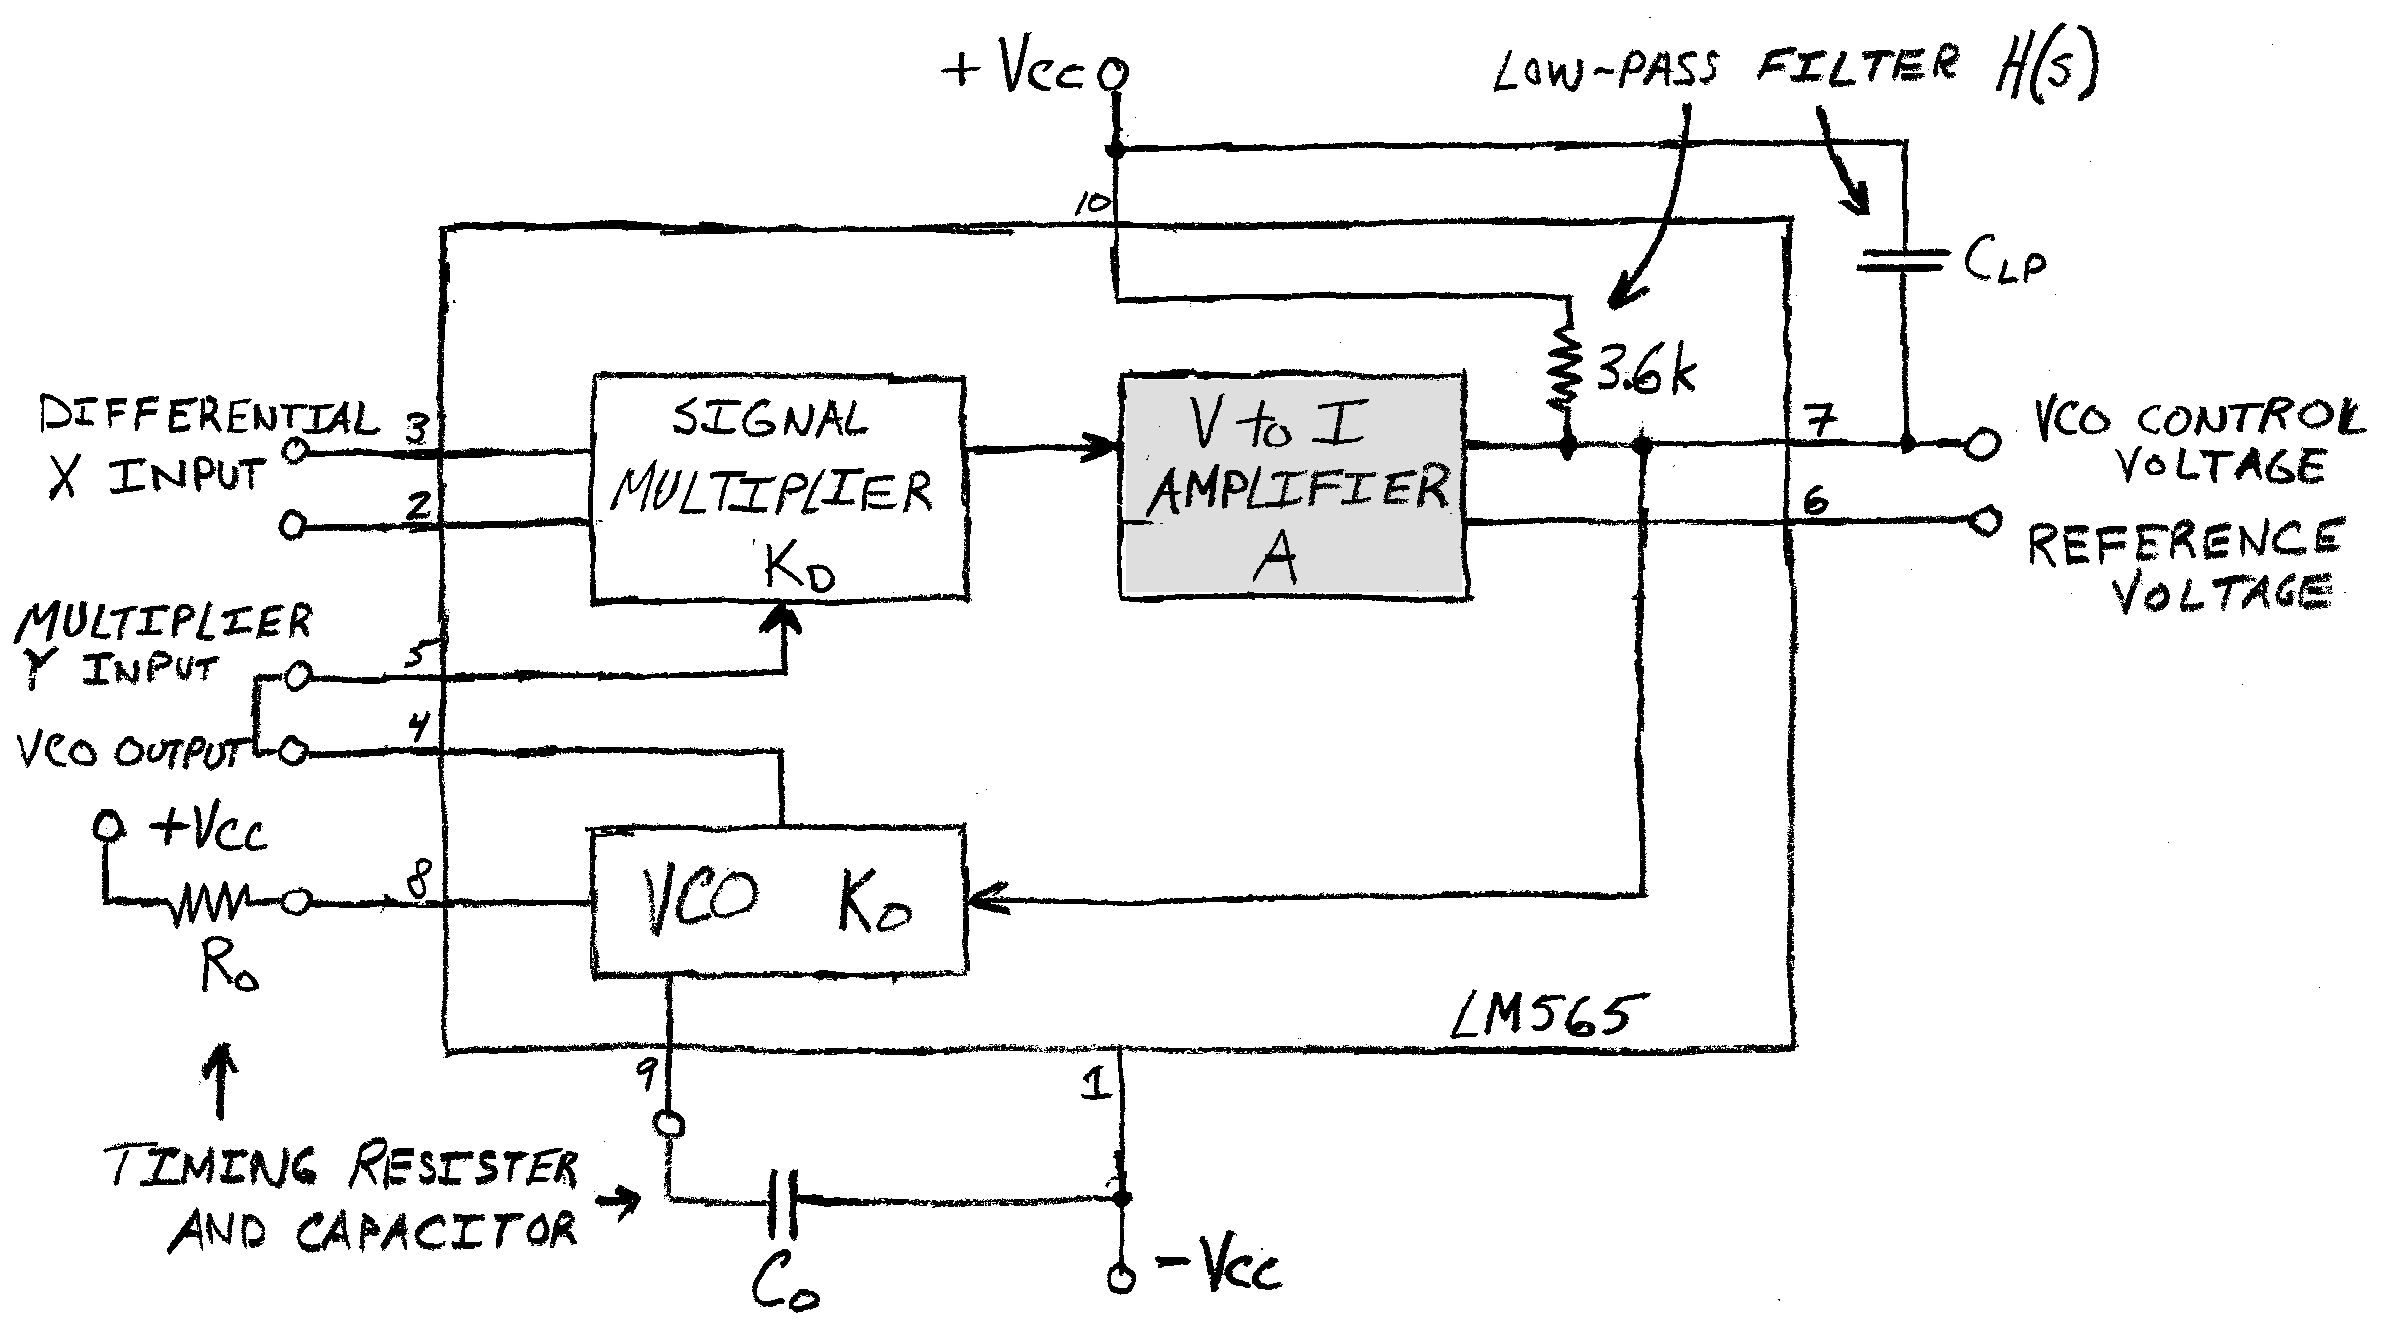
\includegraphics[width=0.75\textwidth]{diagrams/565-block-diagram-i-to-v-amplifier}
	\caption{Role of the Transconductance Amplifier in the LM565 PLL}
	\label{565-block-diagram-i-to-v-amplifier}
\end{figure}

In the circuit schematic for the LM565, the amplifier accepts a voltage from the multiplier and outputs an amplified current signal.
Unlike the original Signetics chip, the low pass filter following the amplifier uses current as the input (R and C are parallel).
A voltage-to-current amplifier is called a transconductance amplifier.

We are doing feedback in the lecture right now, so I decided to implement this module with an opamp and resistive feedback.
Figure \ref{feedback-voltage-amp} shows the block diagram for a feedback amplifier, with an op-amp in the amplifier position.
Note that an op-amp is usually depicted as a voltage-to-voltage amplifier.

\begin{figure}[ht]
	\centering
	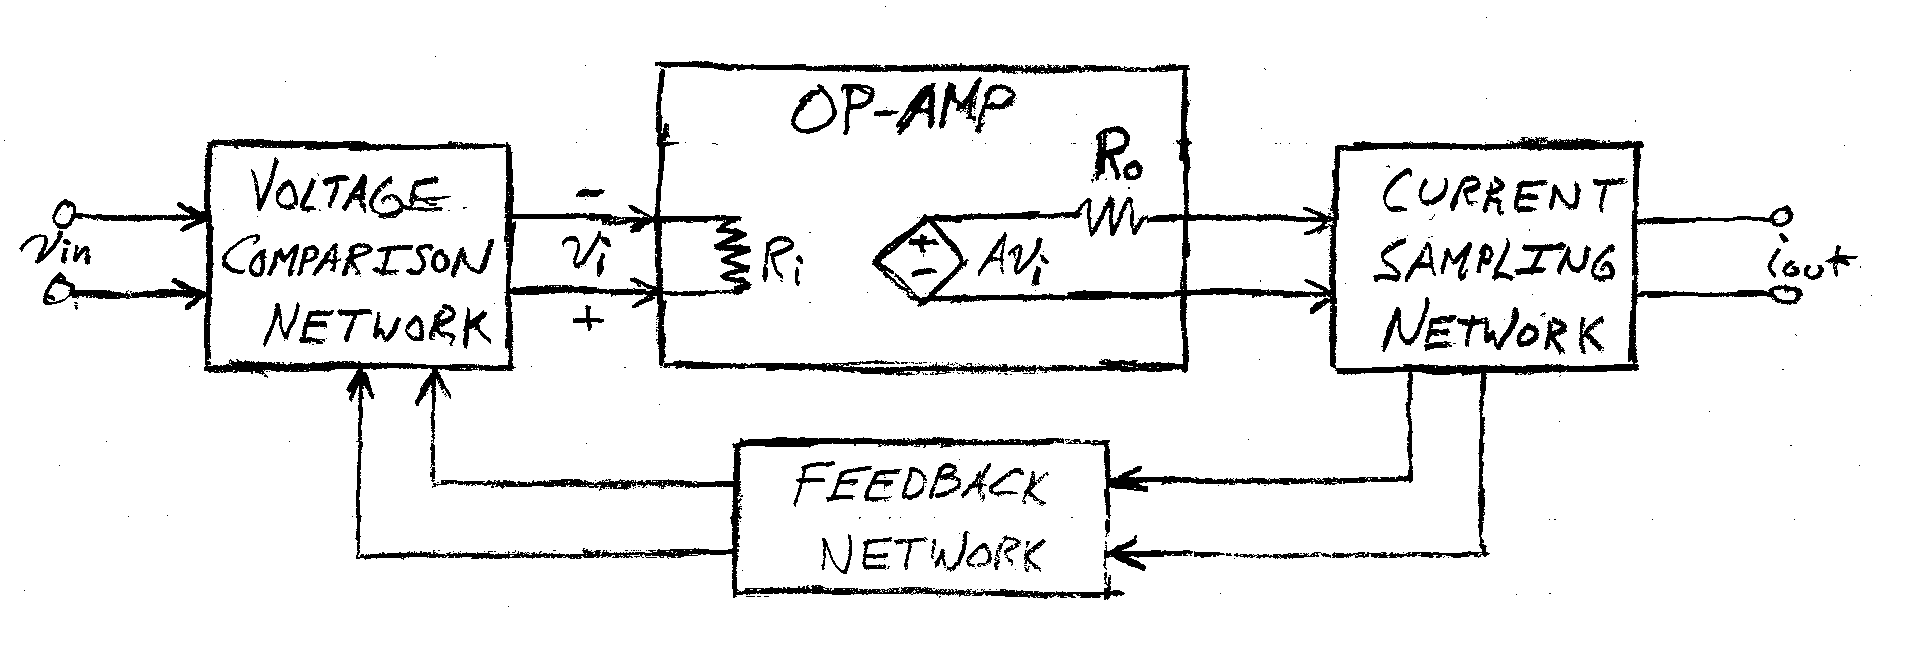
\includegraphics[width=0.75\textwidth]{diagrams/feedback-voltage-amp}
	\caption{Generic Block Diagram of an Op-Amp Feedback Amplifier}
	\label{feedback-voltage-amp}
\end{figure}

We can replace the voltage source in the op-amp with its norton equivalent current source.
Voltage comparison and current sampling are both accomplished with series connections.
Figure \ref{feedback-transconductance-amp} shows these changes, which now depict a transconductance amplifier.

\clearpage

\begin{figure}[ht]
	\centering
	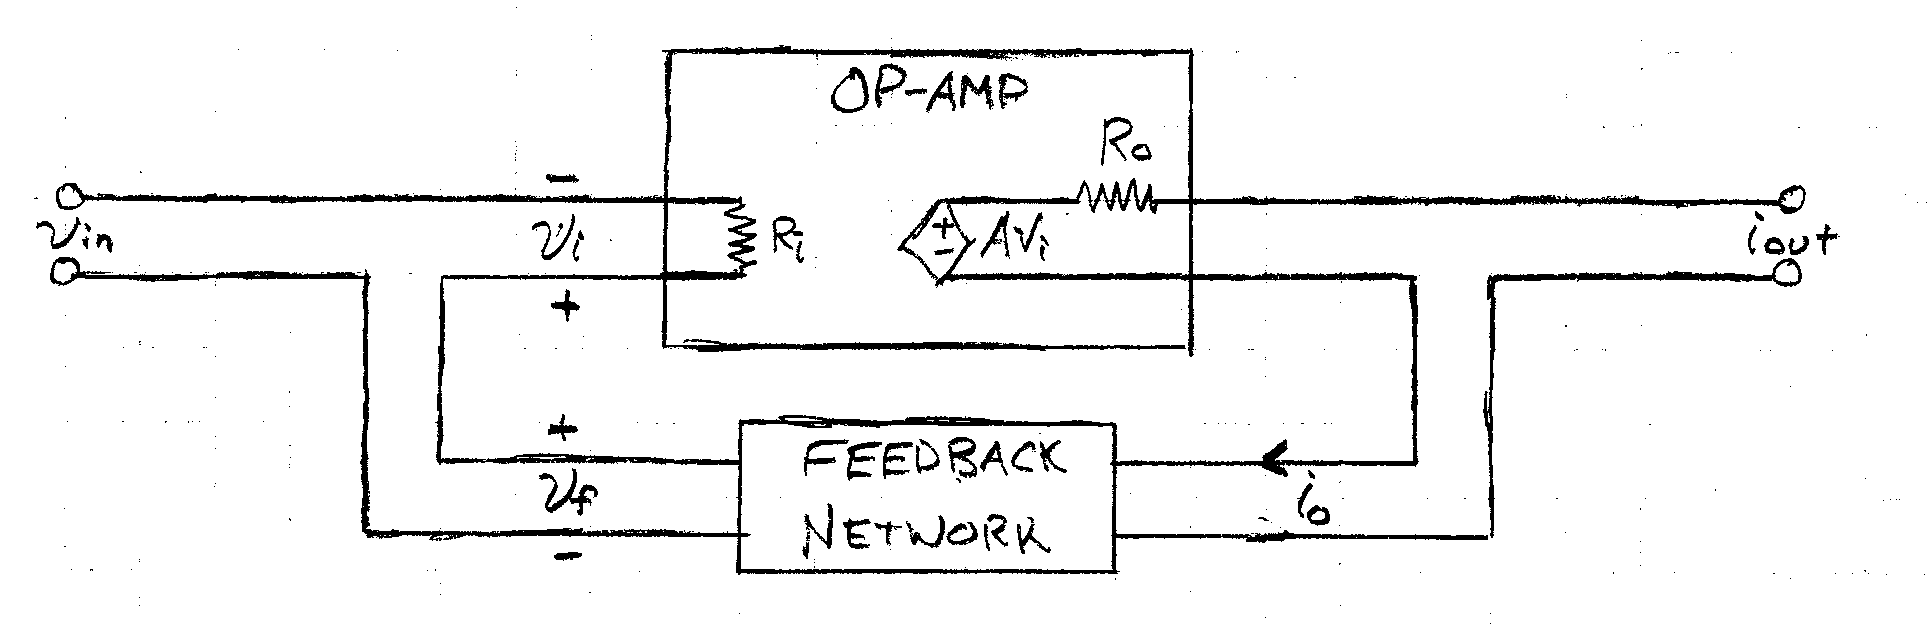
\includegraphics[width=0.75\textwidth]{diagrams/feedback-transconductance-amp}
	\caption{Transconductance Feedback Amplifier Block Diagram}
	\label{feedback-transconductance-amp}
\end{figure}

I tried several feedback networks and eventually settled on one with three resistors; see figure \ref{feedback-network}.

\begin{figure}[ht]
	\centering
	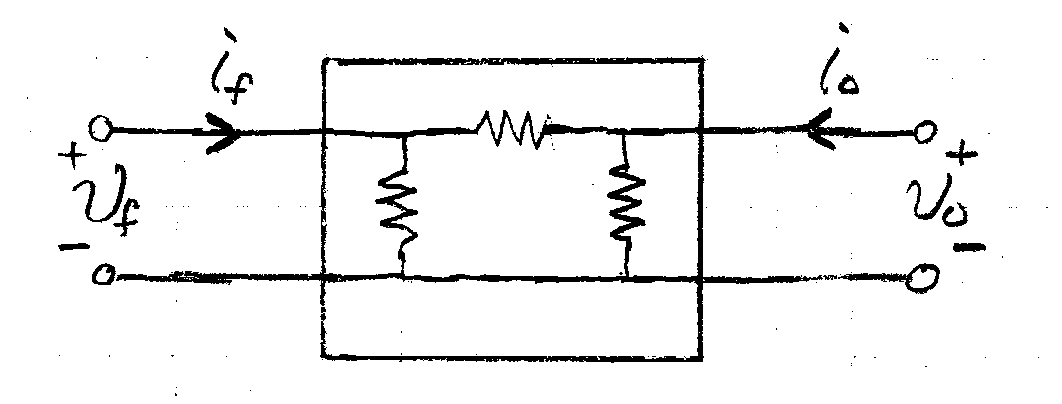
\includegraphics[width=0.35\textwidth]{diagrams/feedback-network}
	\caption{Resistive Feedback Network}
	\label{feedback-network}
\end{figure}

To choose sensible resistors, it is helpful to analyze the feedback network with the h-parameter model.
The dependent sources in the h-parameter model should be comparison and sampling signals, so the matrix should be
\begin{equation*}
\left[ \begin{array}{c}
v_{f}	\\
i_{o}	\end{array}	\right]
=\left[	\begin{array}{cc}
h_{11}	&	h_{12}	\\
h_{21}	&	h_{22}	\end{array}	\right]
\left[	\begin{array}{c}
i_{f}	\\
v_{o}	\end{array}	\right]
\end{equation*}

The h-parameters come out to be
\begin{equation*}
\left[	\begin{array}{cc}
h_{11}	&	h_{12}	\\
h_{21}	&	h_{22}	\end{array}	\right]
=\left[	\begin{array}{cc}
\frac{R_{2}R_{3}}{R_{2}+R_{3}}	&	h_{12}=\frac{R_{3}}{R_{2}+R_{3}}	\\
\frac{R_{2}}{R_{2}+R_{3}}	&	\frac{R_{1}+R_{2}+R_{3}}{R_{1}(R_{2}+R_{3})}	\end{array}	\right]
\end{equation*}

and they correspond to the h-parameter equivalent circuit shown in figure \ref{h-parameter-equivalent-network}.

\begin{figure}[ht]
	\centering
	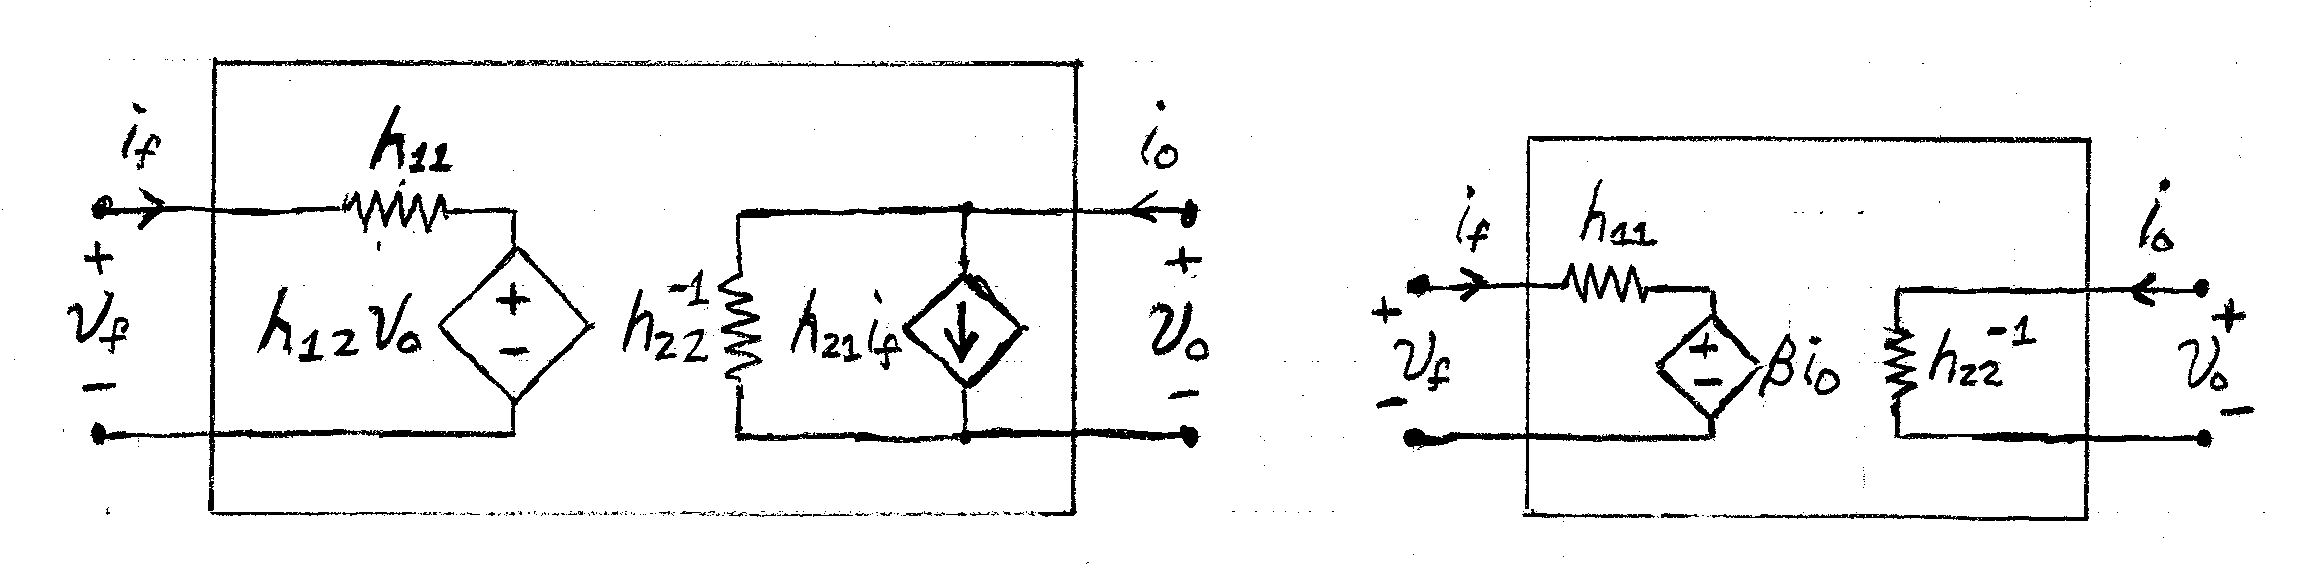
\includegraphics[width=.8\textwidth]{diagrams/h-parameter-equivalent-network}
	\caption{Full h-Parameter Circuit (left) and its Unilateral Approximation (right)}
	\label{h-parameter-equivalent-network}
\end{figure}

An optimal feedback network is unilateral, so $h_{21}$ must be designed to be negligibly small.
\begin{equation}
h_{21}=\frac{R_{2}}{R_{2}+R_{3}}
\label{h21-eq}
\end{equation}

The other value that must be designed is the ratio of the feedback output to the sampled value.
\begin{equation}
\beta=\frac{v_{f}}{i_{o}}
=h_{12}*h_{22}^{-1}
=\frac{R_{3}}{R_{2}+R_{3}}*\frac{R_{1}(R_{2}+R_{3})}{R_{1}+(R_{2}+R_{3})}
\label{beta-design-eq}
\end{equation}

From equation \ref{h21-eq}, it is clear that $R_{2}<<R_{3}$ if we are to neglect the $h_{21}$ crosstalk.
This design decision also allows us to simplify equation \ref{beta-design-eq}.
\begin{equation*}
\beta=1*\frac{R_{1}R_{3}}{R_{1}+R_{3}}
\end{equation*}

If we also design $R_{1}<<R_{3}$, then the feedback ratio is simply
\begin{equation*}
\beta=R_{1}
\end{equation*}

The return ratio for the feedback amplifier is given by
\begin{equation*}
G_{fb}=\frac{G}{1-\beta G}
\end{equation*}

Because the open circuit gain of an op-amp is so large, the return ratio simplifies to
\begin{equation}
G_{fb}=\frac{-1}{\beta}=\frac{1}{R_{1}}
\label{transconductance-gain-eq}
\end{equation}

which is the amplifier gain for the circuit topology shown in figure \ref{transconductance-amplifier-circuit}.

\begin{figure}[ht]
	\centering
	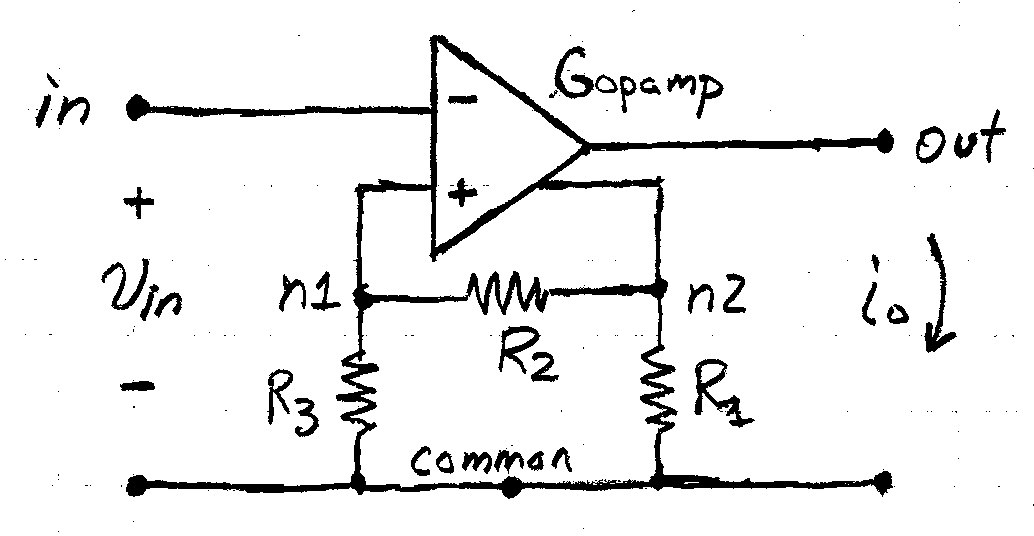
\includegraphics[width=0.4\textwidth]{diagrams/transconductance-amplifier-circuit}
	\caption{Transconductance Amplifier Module}
	\label{transconductance-amplifier-circuit}
\end{figure}


\clearpage
\subsection{Low-Pass Filter}

\begin{figure}[ht]
	\centering
	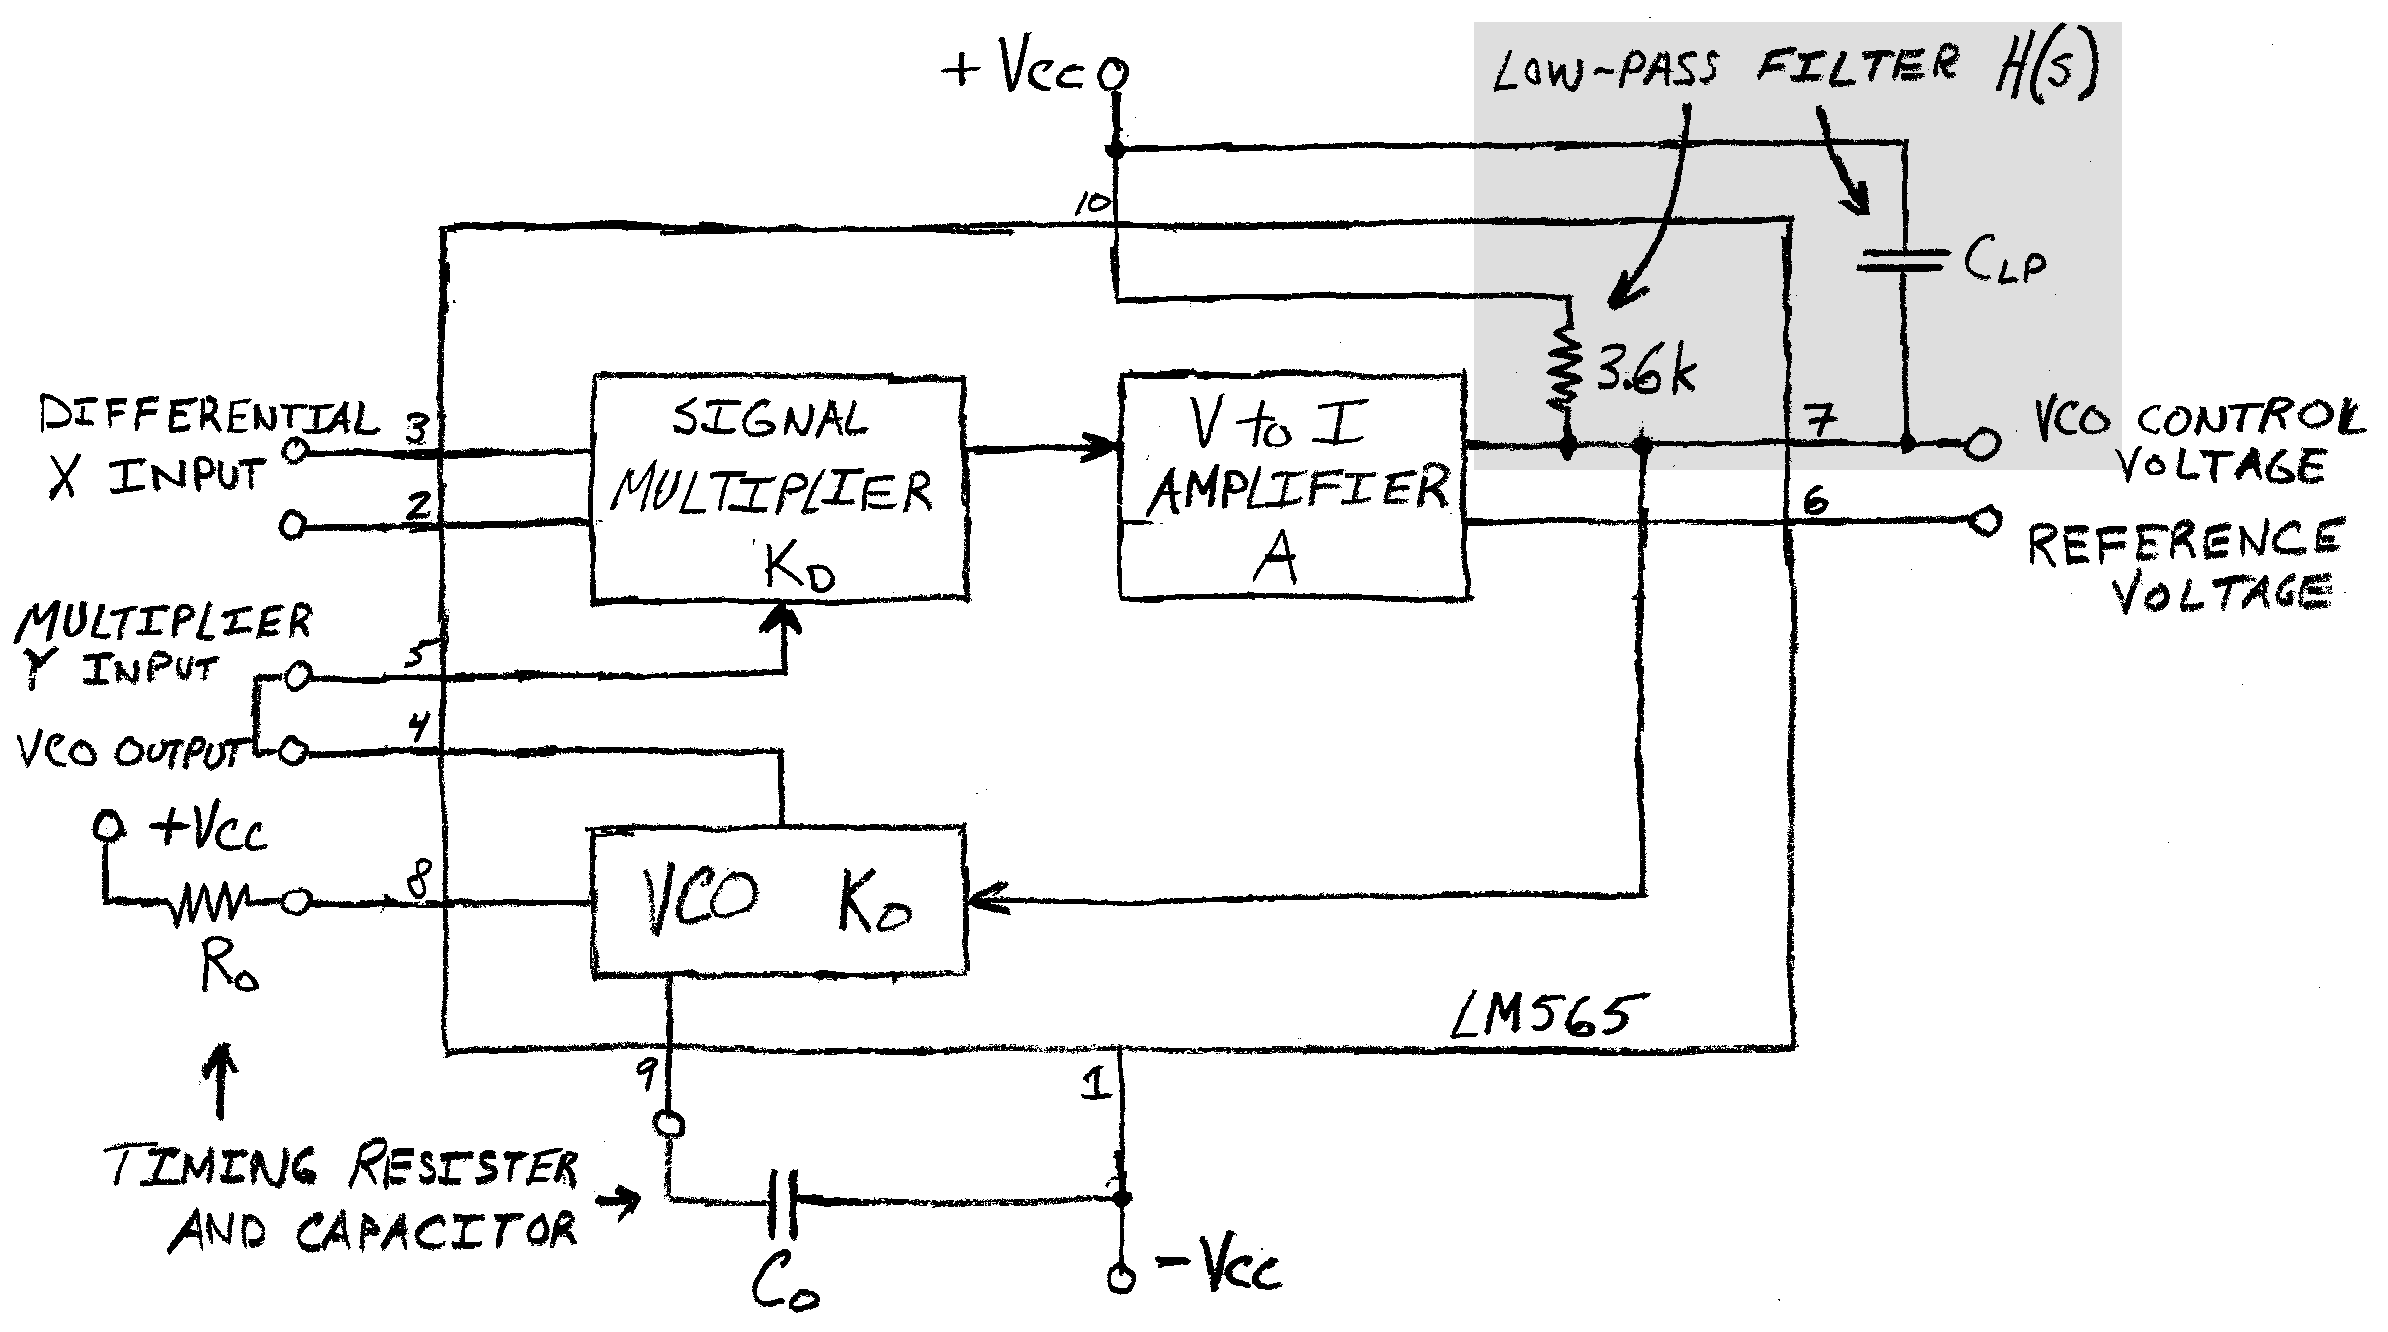
\includegraphics[width=0.75\textwidth]{diagrams/565-block-diagram-low-pass-filter}
	\caption{Role of the Low Pass Filter in the LM565 PLL}
	\label{565-block-diagram-low-pass-filter}
\end{figure}


\section{Design and Simulation}

\subsection{Voltage Controlled Oscillator}

\subsubsection{LM565 vs SPICE Model}

For the timing resistor $R_{0}$, I decided to use $3k\Omega$ because it was available with 1\% tolerance.
Using equation \ref{f0-eq}, the timing capacitors for 1 kHz, 10 kHz, and 100 kHz operating ranges should be
\begin{equation*}
R_{0}=3k\Omega
\end{equation*}
\begin{equation*}
C_{0(1kHz)}=0.1uF \quad | \quad C_{0(10kHz)}=0.01uF \quad | \quad C_{0(100kHz)}=1,000pF
\end{equation*}

\subsubsection{Free Running Frequency, $f_{0}$}

\subsubsection{Oscillator Sensitivity, $K_{O}$}

\subsection{Signal Multiplier}

\subsection{Transconductance Amplifier}

\subsection{Low-Pass Filter}

\subsection{Phase Detector Sensitivity, $K_{D}$}

\subsection{PLL Loop Gain, $K_{O}K_{D}$}

\subsection{FSK Generator}

\subsection{FSK Demodulator}

\begin{figure}[ht]
	\centering
	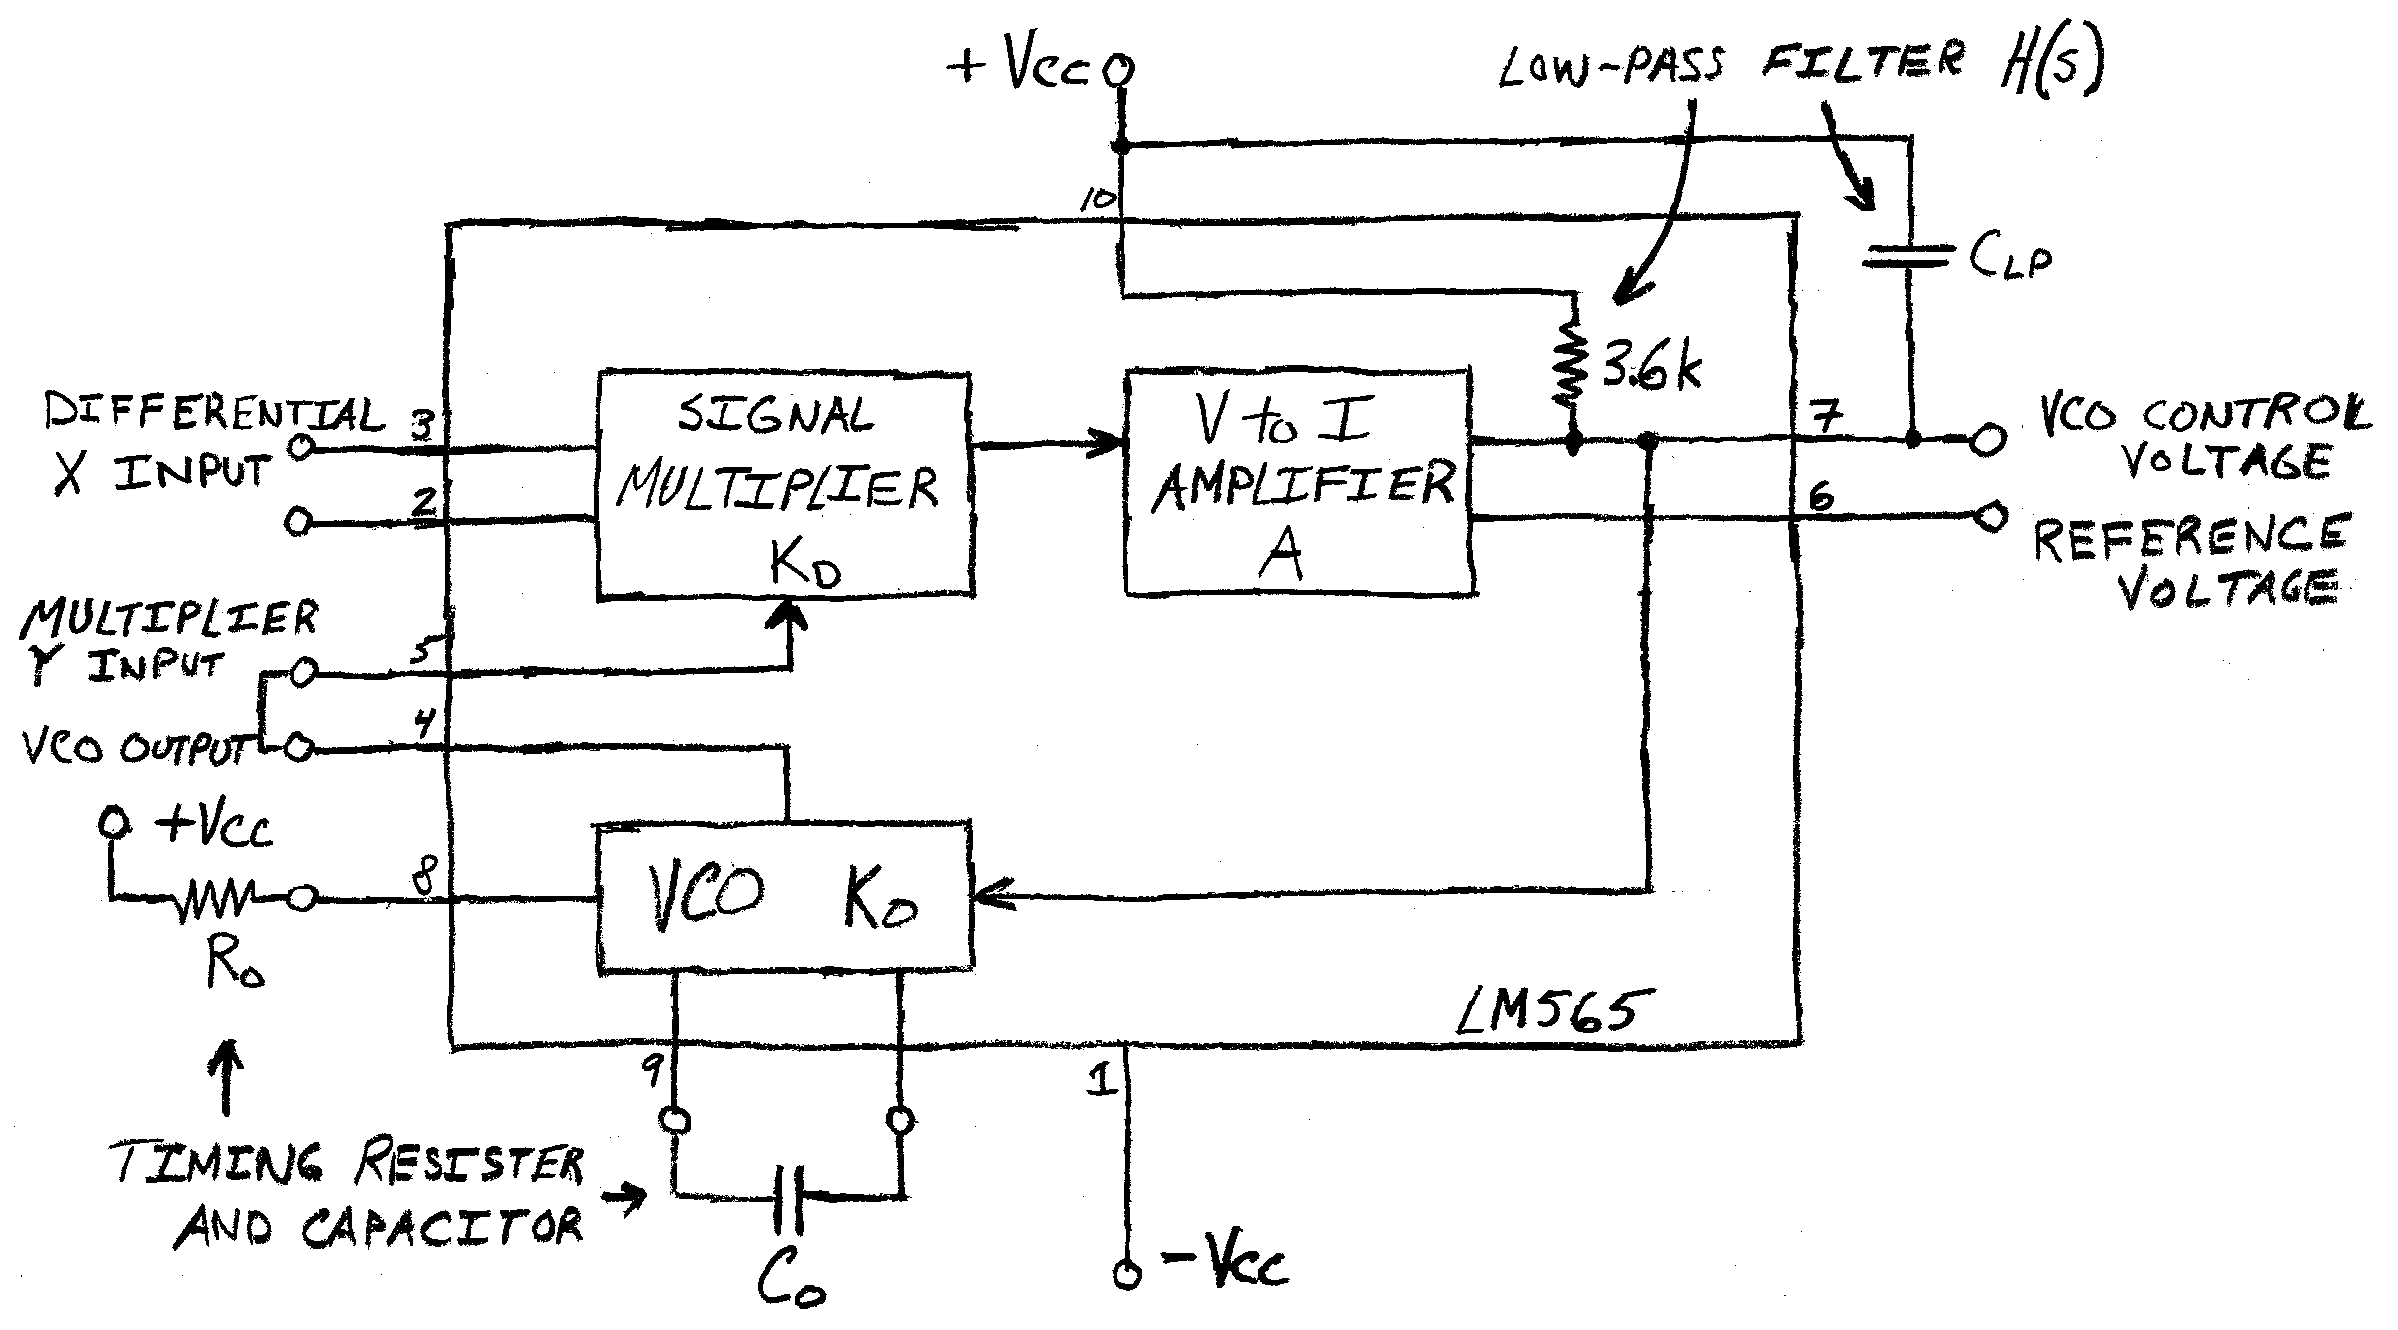
\includegraphics[width=0.75\textwidth]{diagrams/565-block-diagram-additional-c0-port}
	\caption{Block Diagram for Phase Locked Loop SPICE Model}
	\label{565-block-diagram-additional-c0-port}
\end{figure}


\section{Results}

\subsection{Free Running Frequency, $f_{0}$}

\subsection{Oscillator Sensitivity, $K_{O}$}

\subsection{FSK Demodulator}

\section{Conclusions}

\section{Appendices}

\clearpage
\subsection{LM565 Schematic Diagram}
\label{lm565-schematic-diagram}

\begin{figure}[ht]
	\centering
	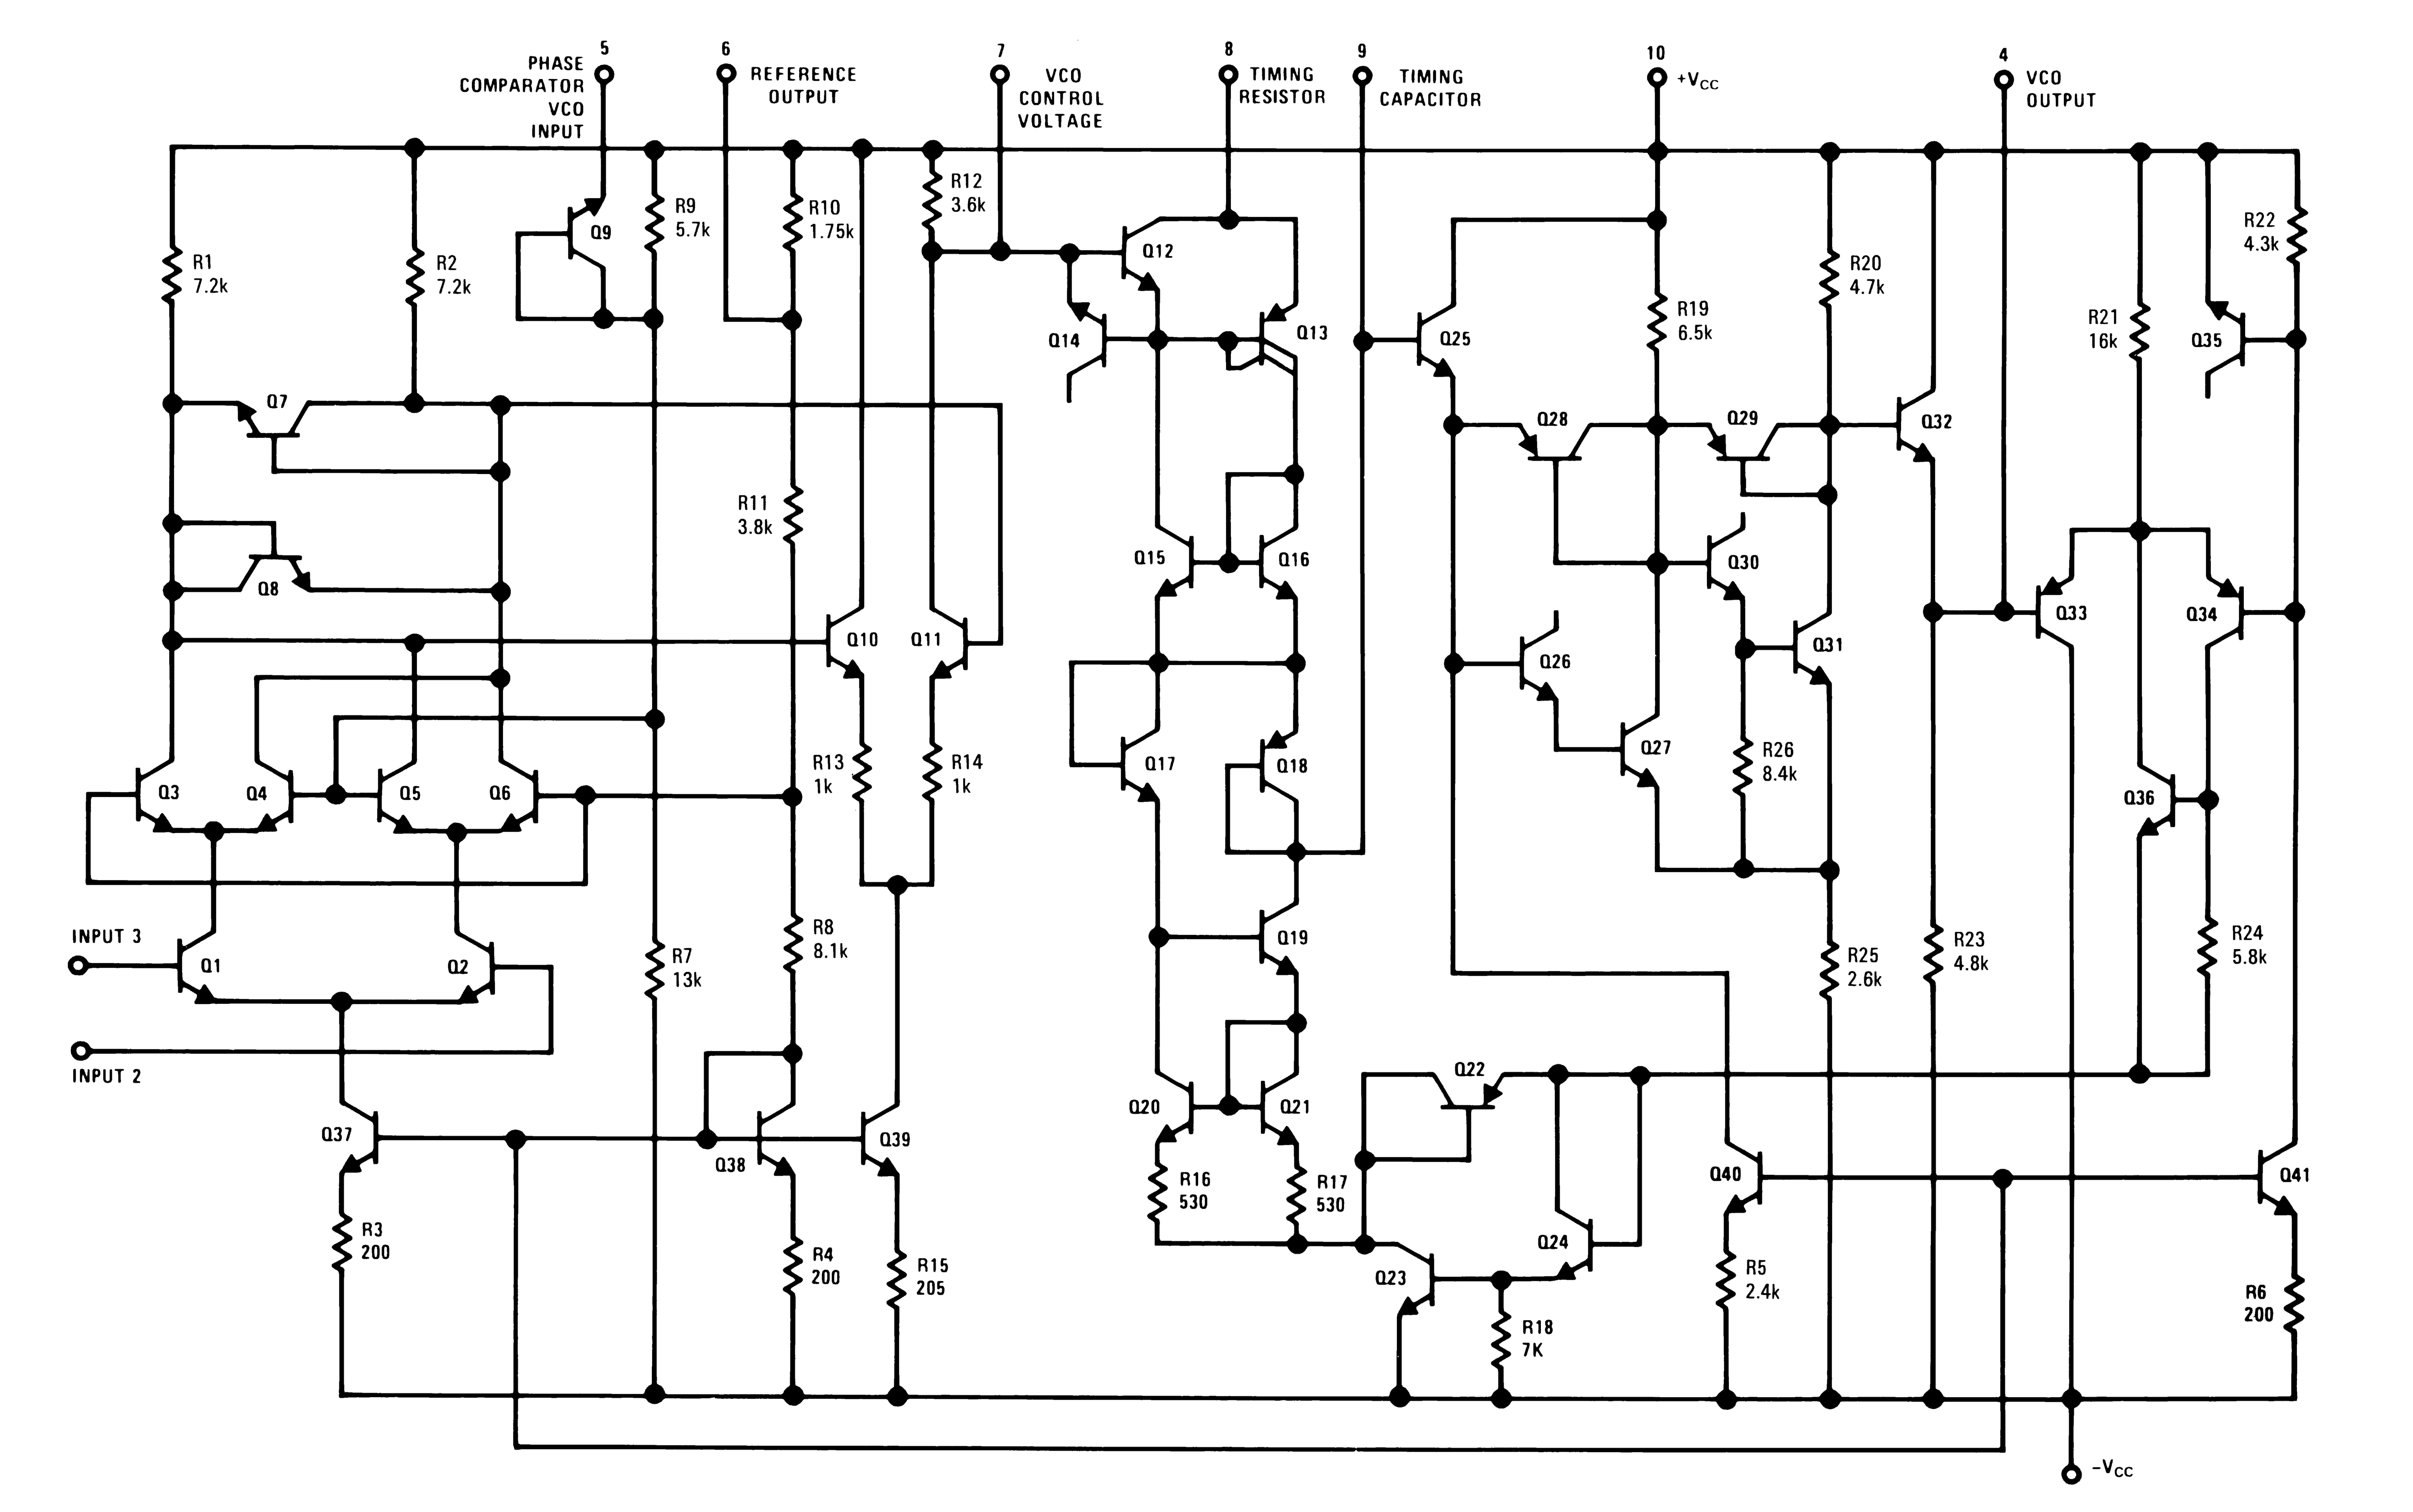
\includegraphics[width=1\textwidth]{diagrams/lm565-equivalent-circuit}
	\caption{LM565 Schematic Diagram; taken from page 6 of the TI datasheet}
	\label{lm565-equivalent-circuit}
\end{figure}

\end{document}
